\chapter[Fundamentação Teórica e Estado da Arte]{Fundamentação Teórica e Estado da Arte}
\label{cha:fundamentacao}
Nessa seção, serão abordados conceitos básicos para a compreensão da monografia (teoria, problema e proposta), começando pela definição de um sinal segundo a literatura, representado por um sinal elétrico, tanto analógico quanto digital; conceituar música e a importância da mixagem realizada por \textit{DJs}, culminando no equipamento utilizado, dando enfoque ao \textit{mixer}, seja na sua história, evolução e no seu estado da arte.

\section{Sinal: Conceito}

\begin{citacao}
"Os sinais, que são funções de uma ou mais variáveis independentes, contêm informações sobre o comportamento ou natureza de algum fenômeno, enquanto os sistemas respondem a algum sinal em particular, produzindo outros sinais ou algum comportamento desejado." \cite{oppenheim2010sinais}.
\end{citacao}

Como exemplifica \cite{oppenheim2010sinais}, tensões e correntes ao longo do tempo são funções, ou seja, sinais, enquanto o circuito em si pode ser compreendido como um sistema que reage à entrada aplicada, ao produzir sinais de saída.

Sensores são dispositivos capazes de mensurar grandezas físicas através da captação de sinais elétricos. Dessa forma, a criação desses instrumentos permitiu a compreensão de fenômenos físicos. Assim, o monitoramento de grandezas permite que se atue em sistemas físicos a fim de se obter um resultado desejado.

Com o desenvolvimento de sensores na história da instrumentação, foi possível a obtenção da quantização de parâmetros físicos através de sinais elétricos. Dessa forma, a compreensão de fenômenos físicos e, consequentemente, a construção de sistemas que podem alterar os sinais conforme a resposta desejada.

\section{Sinal Contínuo}
Um sinal pode ser classificado como contínuo caso sua variável independente seja contínua, ou seja, se houver um valor para cada instante de tempo (variável independente).

\begin{figure}[h]
	\centering
	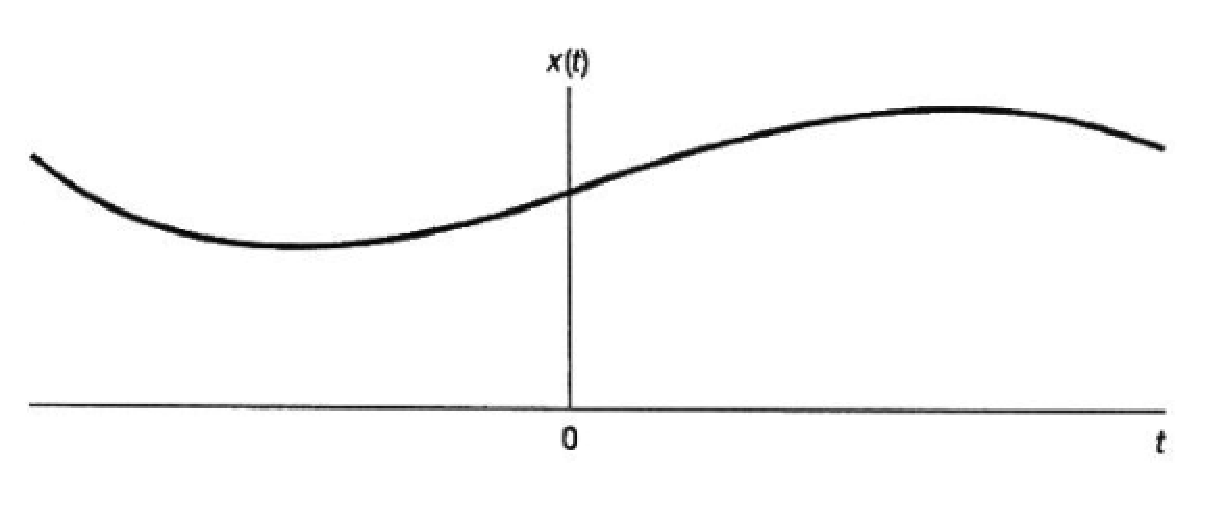
\includegraphics[scale=0.5]{figuras/fig01.eps}
	\caption{sinal de tempo contínuo \cite{oppenheim2010sinais}}
	\label{fig01}
\end{figure}

Por exemplo, na Figura \ref{fig01}, entre o intervalo de 0 a \textit{t}, há infinitos valores tanto de tempo quanto para o parâmetro em função do tempo \cite{oppenheim2010sinais}. Um exemplo pode ser o valor de corrente em um resistor alimentado por uma tensão ou um som que gera uma pressão acústica no ar captada pelo sistema auditivo. A Figura \ref{fig01} é um exemplo de um gráfico para um sinal contínuo no tempo. 


\subsection{Sinal Discreto}
No caso de um sinal discreto, a sua variável independente é o tempo discreto, que pode ser definido por um conjunto de números inteiros, de forma que caso \textit{n} não seja inteiro, não há valor definido. 

\begin{figure}[h]
	\centering
    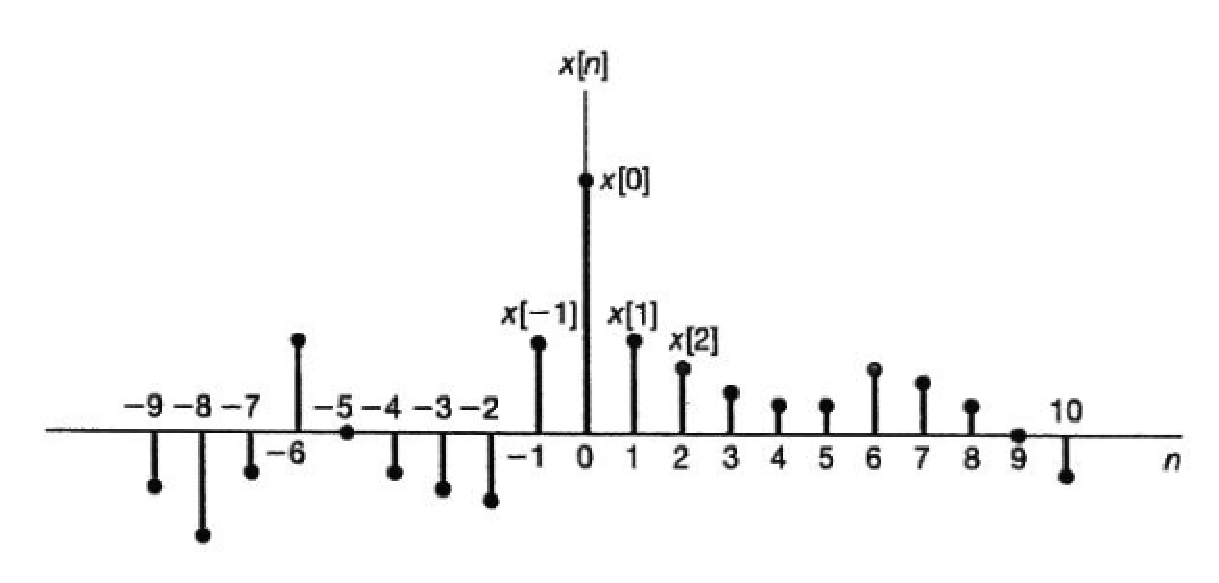
\includegraphics[scale=0.5]{figuras/fig02.eps}
	\caption{sinal de tempo discreto \cite{oppenheim2010sinais}}
	\label{fig02}
\end{figure}

Dessa forma, entre as amostras consecutivas da Figura \ref{fig02}, não há infinitos valores como há no tempo contínuo.

\subsection{Transformada de Fourier}
Uma ferramenta matemática crucial para a análise de sinais na frequência é a transformada de Fourier, que realiza uma modificação do termo independente, saindo do tempo ou espaço e indo para frequências, também denominada de equação de análise, que pode ser visualizada na equação \ref{eq:03}.

\begin{equation}  \label{eq:03}
X(e^{j\omega})= \sum_{n=-\infty}^{+\infty} x[n]e^{-j\omega n}
\end{equation}

\begin{equation}  \label{eq:04}
x[n]=\frac{1}{2\pi} \int_{2\pi}^{} X(e^{j\omega})e^{j\omega n} \,d\omega
\end{equation}

De forma análoga, a transformada inversa, ou a também chamada de equação de síntese, realiza o processo inverso, modificando o sinal representado no domínio da frequência para o seu domínio original, segundo \cite{oppenheim2010sinais}, seja tempo ou espaço. A equação da transformada inversa pode ser visualizada na equação \ref{eq:04}

\subsection{Teorema da Amostragem}
Devido ao desenvolvimento da computação nas últimas décadas e pela consequente diminuição de custos de produção e de aquisição de dispositivos capazes de realizar o processamento digital de sinais, tornou-se muito vantajoso a utilização de sinais no tempo discreto, para que possam ser trabalhados digitalmente e, posteriormente, ou não, serem convertidos novamente para o tempo contínuo, sem a perda da informação inicial. 

O processo de obter um sinal discreto a partir de um sinal contínuo é denominado amostragem, e para que, a partir do sinal amostrado, reconstrua-se o sinal contínuo original, o sinal e o processo de amostragem devem preencher alguns requisitos.

Para que um sinal seja amostrado, é necessário que o intervalo de amostragem, ou seja, o espaçamento entre duas amostras, seja regular. A cada período $T$, uma amostra é adquirida, resultando em uma frequência de amostragem $f = 1/T$. Ao passar essa função do domínio do tempo para o domínio da frequência, obter-se-á uma banda de frequências que compõe o sinal no domínio do tempo.

\begin{figure}[h]
	\centering
    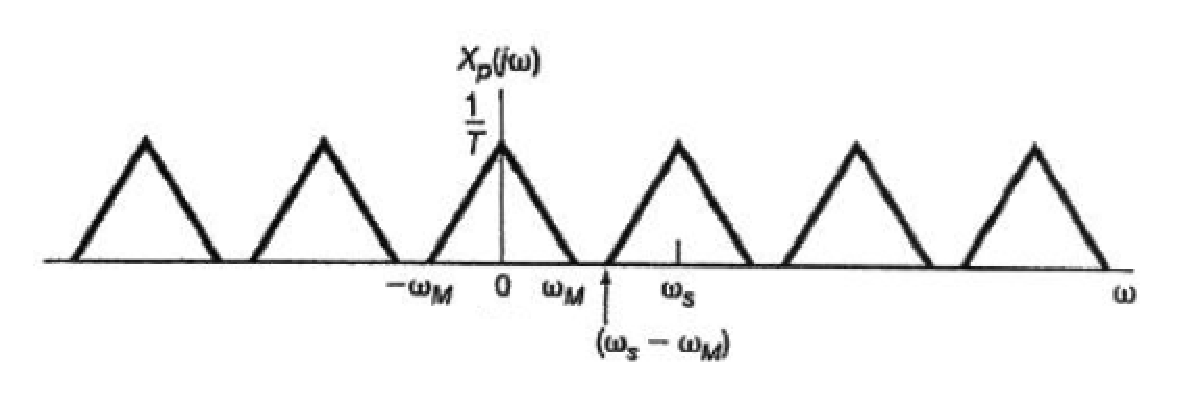
\includegraphics[scale=0.5]{figuras/fig03.eps}
	\caption{espectro do sinal amostrado com $W_s > 2W_m$ \cite{oppenheim2010sinais}}
	\label{fig03}
\end{figure}

Ao observar a Figura \ref{fig03}, sendo a componente $\omega_M$ a maior frequência angular presente no sinal do tempo, $\omega_s$ a frequência de amostragem, constata-se que $\omega_M < (\omega_s - \omega_M)$ segundo Oppenheim e Willsky \cite{oppenheim2010sinais}. Dessa forma, $\omega_s > 2\omega_M$. Caso a frequência de amostragem seja menor que $\omega_M$, haverá sobreposição das bandas adjacentes e, por conseguinte, a reconstrução do sinal não será possível. Ao respeitar esse requisito, o sinal pode ser recuperado ao utilizar um filtro passa-baixas com a frequência de corte maior que $\omega_M$ e menor que $\omega_M - \omega_s$.
Essa análise é o Teorema da Amostragem que infere que a:

\begin{equation} \label{eq:01}
\omega_s > 2\omega_M
\end{equation}

em que

\begin{equation} \label{eq:02}
\omega_s = \frac{2\pi}{T}
\end{equation}

O parâmetro $\omega_M$, que deve ser menor que metade da frequência de amostragem $\omega_s$, recebe o nome de frequência de Nyquist \cite{oppenheim2010sinais}.
\par
Esse teorema foi explicitado na literatura por Shannon \cite{Shannon}, mas foi apontado anteriormente por Nyquist \cite{nyquist}. A partir dele, compreende-se a suficiência da representação de um sinal pela série de Fourier por 2TW amostras, no qual T é a duração de uma função e W é a frequência mais alta que compõe o sinal.

\subsection{\textit{Aliasing}}
Quando a frequência de amostragem não está de acordo com o critério de Nyquist, ou seja, menor que o dobro da frequência mais alta, não se tem a reconstrução do sinal, já que, ao realizar a filtragem passa-baixa, na banda $\omega_M$ haverá componentes da banda adjacente.

\subsection{Teorema da Quantização}

Após a amostragem de sinais, obtém-se um conjunto de sinais. Para que esses sinais, pertencentes ao domínio contínuo, possam ser processados, é necessário que se faça a quantização digitalmente. A quantização é um processo no qual se determina intervalos de valores, atribuindo cada valor amostrado a um valor quantizado em função do intervalo no qual o valor se insere. Para cada sinal amostrado, é atribuído um valor quantizado.

\begin{figure}[h]
	\centering
    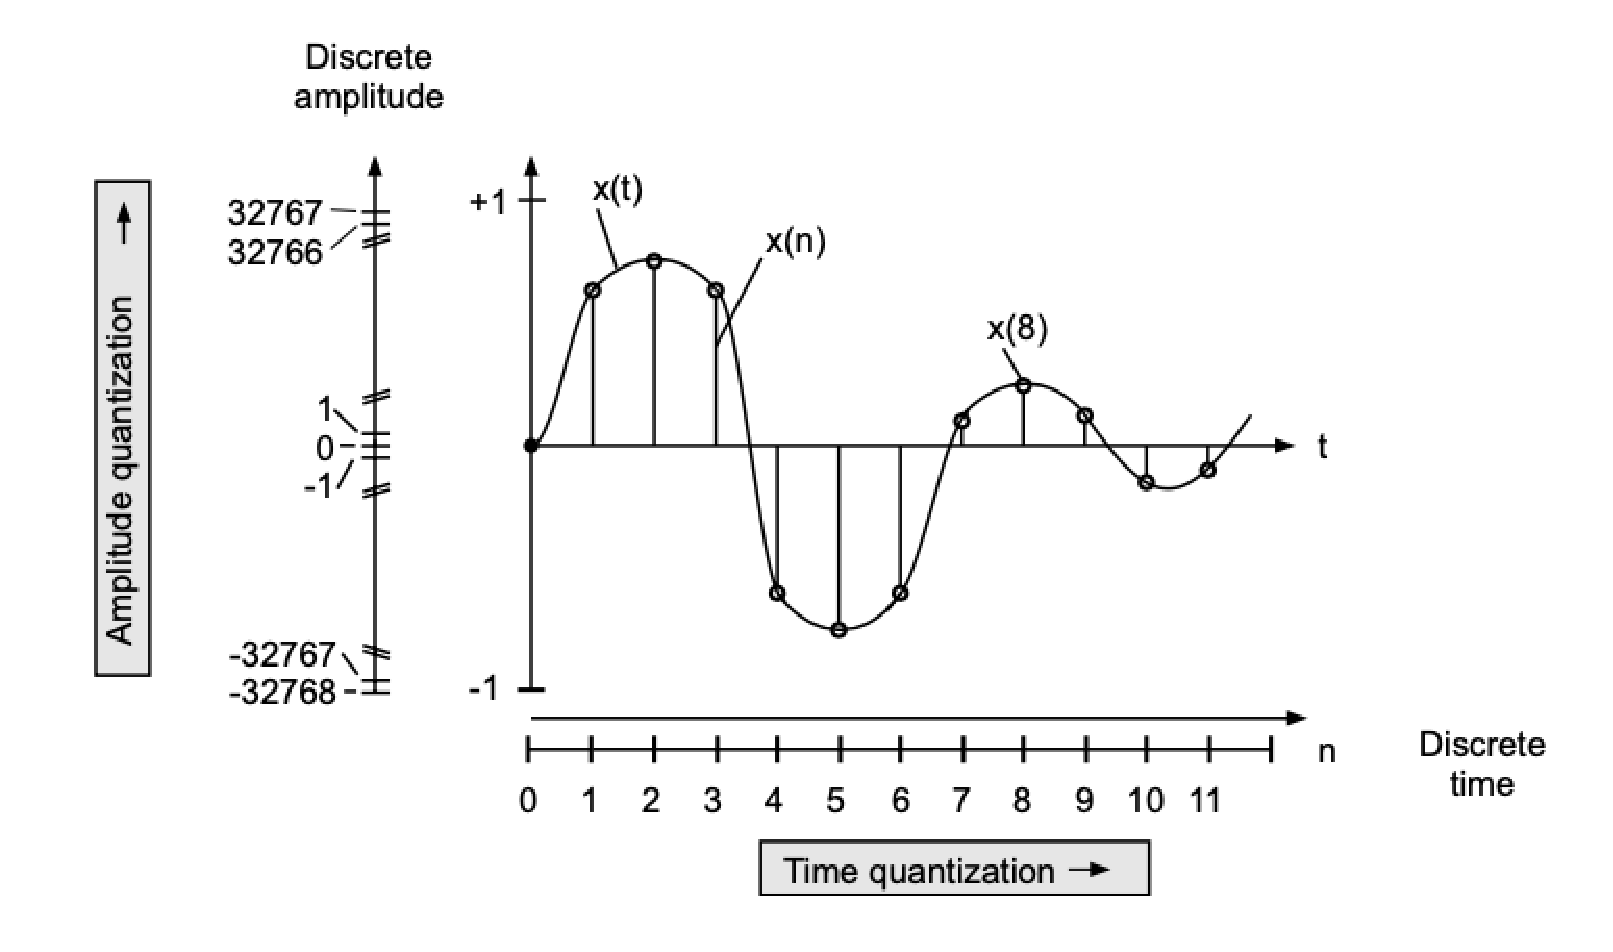
\includegraphics[scale=0.4]{figuras/fig04.eps}
	\caption{quantização de amplitudes em tempo discreto \cite{oppenheim2010sinais}}
	\label{fig04}
\end{figure}

Para determinar com precisão os valores dos intervalos da quantização, o maior e o menor valor obtido pós-amostragem são os limites dos valores de amplitudes discretos. Na Figura \ref{fig04}, observa-se o processo a partir do qual, para cada valor obtido na amostragem, há um intervalo correspondente que passará a representar esse sinal.
\par O intervalo de amplitude discreta da Figura \ref{fig04} varia de -32768 a +32767, totalizando 65536 possíveis amplitudes discretas, ou seja, $2^{16}$ possíveis amplitudes. Dessa forma, cada amplitude pode ser representada por uma palavra binária de 16 \textit{bits}. A quantidade de \textit{bits} a ser utilizada determinará a quantidade de intervalos possíveis, o que, por conseguinte, determinará a precisão da quantização, devido a um erro gerado.
\par Cada processo de quantização deve levar em conta a precisão necessária e os limites do intervalo de valores possíveis. Ao final, o procedimento de quantização é essencial para as conversões AD (analógico para digital).

A quantização, o processo de digitalizar a amplitude, é descrita pelo Teorema de Quantização de Widrow \cite{widrow}, segundo Zölzer \cite{zolzer2008digital}.

\section{Som e Música}
Nesta seção, será apresentada uma abordagem histórica, conceitual e técnica sobre a natureza do som e a mixagem realizada por um \textit{DJ}. A partir do som, a música será definida e grandezas físicas serão abordadas. Posteriormente, serão discutidos cenários históricos e técnicos sobre o início das gravações musicais e da discotecagem. Em seguida, com um enfoque mais atual, será apresentado um contexto contemporâneo acerca da mixagem realizada por um \textit{DJ}, que realiza uma seleção musical com base nas características de cada música e faz transições para criar uma experiência musical única.

\subsection{Conceito físico}
Segundo Moyses \cite{moyses}, "... corpos em vibração produzem sons ...". Dessa forma, é necessário que haja um meio para que o som se propague. Esse meio pode ser líquido, viscoso, sólido ou gasoso (como a atmosfera). De acordo com o mesmo autor, "... ondas sonoras na atmosfera são ondas longitudinais, associadas a variações de pressão, ou seja, compressões e rarefações ...". \par Dessa forma, a oscilação de um objeto provoca constantemente compressão e rarefação, alterando a densidade na camada adjacente ao meio pelo qual o som será transmitido e gerando uma diferença de pressão que causa um deslocamento adjacente. Portanto, o ciclo de propagação de um som pode ser visualizado na Figura \ref{fig07}.

\begin{figure}[h]
	\centering
    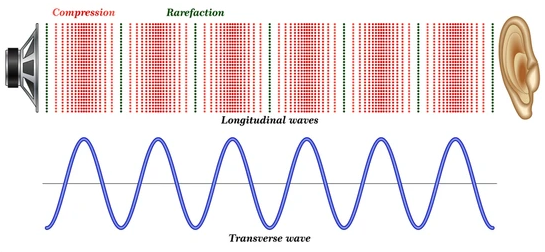
\includegraphics[scale=0.6]{figuras/fig07.png}
	\caption{ciclo de propagação do som \cite{shutterstock}}
	\label{fig07}
\end{figure}

Conforme indica Moyses \cite{moyses}, há parâmetros quantitativos que influenciam a percepção auditiva: intensidade, altura e timbre. A intensidade se relaciona com a amplitude da onda sonora. A altura se refere à banda na qual o som está localizado, seja nas frequências baixas (características graves) ou nas altas frequências (características agudas), em relação à faixa de frequência audível pelo ouvido humano. Já o timbre são sons que possuem a mesma frequência principal, que o autor chama de "tom fundamental da frequência", mas que possuem outras componentes em frequências superiores, tornando o som reconhecível, apesar de ter o mesmo tom fundamental.

\subsection{Audição Humana}
Como Farnell observa \cite{farnell}, embora o corpo humano possa sentir vibrações de 1 a 20 Hz, o ouvido humano é capaz de perceber sons a partir de 20 Hz até 10 kHz ou 20 kHz, dependendo da idade do ouvinte. A faixa normal na qual a voz humana se localiza está entre 300 e 3000 Hz; no entanto, harmônicos provenientes de sons reais podem superar esse limite, inclusive ultrapassando os 20 kHz. Dessa forma, ao utilizar o Teorema de Amostragem, presume-se que a taxa de amostragem mínima necessária para a reconstrução perfeita de um som amostrado seja de, no mínimo, 40 kHz.

\subsection{História da Gravação e Reprodução de Som}
A partir do som, a humanidade foi capaz de criar uma expressão artística denominada música, que permite a expressão de ideias, sentimentos, identidades culturais e formas de entretenimento. Além disso, a evolução da tecnologia no século XX proporcionou uma grande difusão da música devido às novas possibilidades de gravação e reprodução. \par
O marco inicial da gravação de som é atribuído a Thomas Edison, conforme Roads \cite{roads1996computer}, que inventou o fonógrafo em 1877. Ao longo da história, a forma de gravação, armazenamento e reprodução de música foi aperfeiçoada, passando por gramofones, gravadores de fios, fita magnética e vinil. Esses dispositivos utilizavam gravação analógica. \par
O primeiro formato digital amplamente utilizado foi o CD. Outros formatos digitais tentaram alcançar a mesma popularidade do CD, como o MiniDisc, DVD de áudio e Blu-Ray áudio; no entanto, somente os arquivos digitais, com destaque para o MPEG-2 Audio Layer III, mais conhecido como MP3, conseguiram alcançar e superar a popularidade do CD. Esse sucesso deve-se ao uso eficiente de métodos de compressão e compartilhamento, que possibilitaram ao MP3 se tornar o principal meio de compartilhamento de música, acompanhando a ampliação do acesso a computadores e dispositivos digitais capazes de reproduzir música de forma acessível.

\subsection{Disc Jockeys \textit{DJs}}

Cada novo formato de mídia possibilitou novas formas de circulação da música. Cada mudança de formato provocou uma transformação na forma como a música é apreciada, começando com apresentações ao vivo, passando por reproduções via rádio, e culminando na reprodução em qualquer lugar com um aparelho adequado. Isso levou ao surgimento de especialistas em curadoria musical, que influenciaram e modificaram o consumo de música ao transmitir músicas a partir de vinis.

Segundo Brewster e Broughton \cite{lastnight}, houve uma grande luta para que \textit{DJs} que transmitiam suas seleções nas rádios recebessem apoio das gravadoras. Após a Segunda Guerra Mundial, a Capital Records formalizou esse apoio ao reconhecer o potencial de divulgação dos \textit{DJs}s em rádios. O sucesso desses \textit{DJs}, que influenciavam a população das regiões cobertas por suas rádios, teve a capacidade de desenvolver novos gêneros e tendências, pois eram criadores de tendências.

Em 1943, Jimmy Savile observou que um amigo havia conseguido conectar a saída de um gramofone a um rádio valvulado, transformando-o em uma saída de áudio. Isso inspirou Savile a criar um pequeno salão de dança onde gravações de jazz seriam tocadas, permitindo que as pessoas dançassem sem a presença de uma banda. Assim, nasceu um clube, conforme relatado por Brewster e Broughton \cite{lastnight}. Em seu segundo evento, Savile substituiu o rádio valvulado por um alto-falante. Com o aumento do público, ele implementou essa ideia em vários clubes na Inglaterra e, em um projeto específico, teve a ideia de usar dois toca-discos para diminuir o tempo de transição entre as músicas.

Em 1957, conforme Brewster e Broughton \cite{lastnight}, Bob Casey promovia festas em ginásios escolares usando um toca-discos conectado a um pequeno alto-falante. Utilizando o sistema de áudio do ginásio, ele posicionava um microfone na saída do alto-falante e transmitia o som amplificado pelo sistema de áudio. Seu pai, um engenheiro de som, desenvolveu um sistema em 1955 com dois toca-discos e controle de volume, permitindo a comutação entre discos e comentários enquanto o volume da música era reduzido.

De acordo com Brewster e Broughton \cite{lastnight}, em 1964, durante a Feira Mundial em Nova Iorque, Alex Rosner apresentou o primeiro sistema estéreo com dois canais de áudio, um avanço significativo na experiência de audição. Inspirados em sistemas de som da Broadway, David Mancuso e Alex Rosner criaram, para o The Loft (uma famosa festa alternativa), um sistema de som com \textit{subwoofers} (alto-falantes dedicados aos tons graves) e \textit{tweeters} (alto-falantes dedicados aos médios).

Em 1971, Alex Rosner desenvolveu o primeiro \textit{mixer} estéreo para \textit{DJs}, o Rosnie, para o Haven Club (um clube famoso da época), como ilustrado na Figura \ref{fig08}. Esse equipamento contava com duas saídas: uma para fones de ouvido e outra para as caixas de som, permitindo a seleção independente de canais para o retorno da música ao \textit{DJ} e a saída principal. Além disso, o controle \textit{on/off} também foi implementado para o microfone.

\begin{figure}[h]
	\centering
    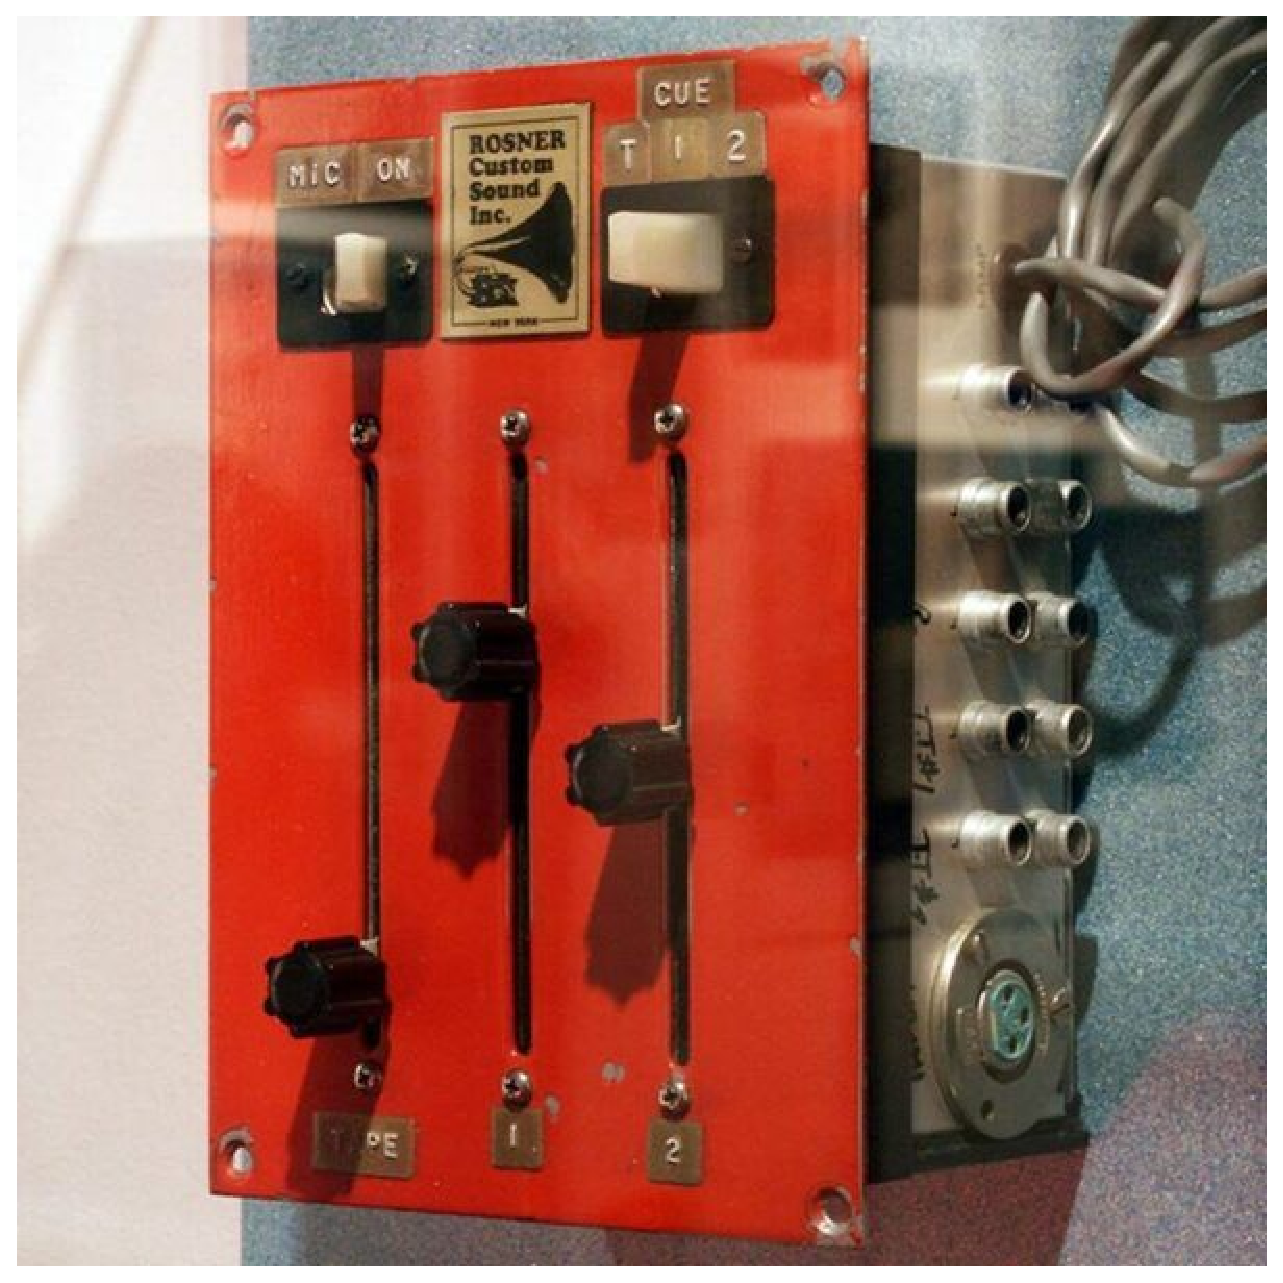
\includegraphics[scale=0.4]{figuras/fig08.eps}
	\caption{Rosnie - inventado por Alex Rosner \cite{stoneyroadsStoryBehind}}
	\label{fig08}
\end{figure}

O Rosnie foi o primeiro \textit{mixer} para aplicações fora de estúdios a controlar o ganho de bandas de frequência. Ao contrário das soluções anteriores que apenas controlavam o volume dos canais, esse equipamento permitiu mixar dois discos simultaneamente de forma que as transições entre músicas fossem extremamente suaves, muitas vezes não se percebendo a transição entre uma música e outra. No entanto, esse equipamento não foi criado com fins comerciais.

Louis Bozak, auxiliado por Alex Rosner, criou o CMA-10-2DL em 1971, visto na Figura \ref{fig10}, o primeiro \textit{mixer} estéreo comercializado que instantaneamente se tornou padrão nos clubes da época.

\begin{figure}[h]
	\centering
    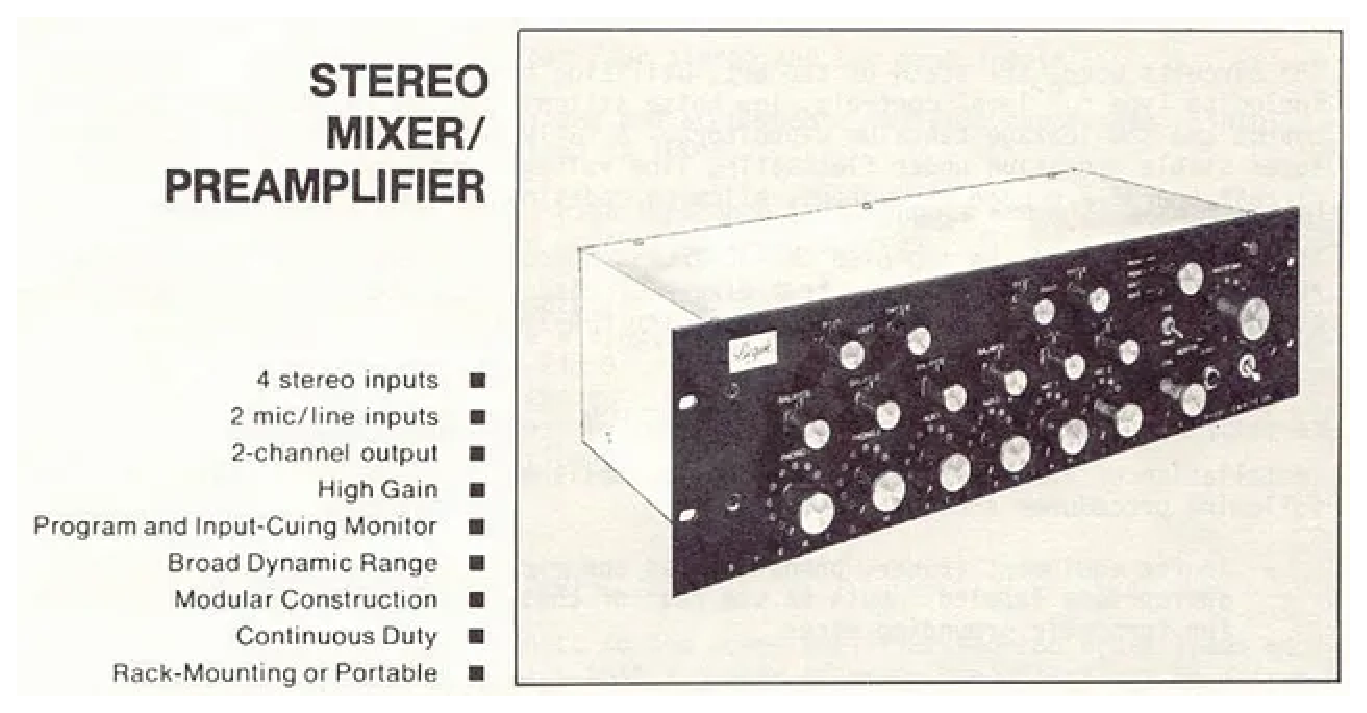
\includegraphics[scale=0.6]{figuras/fig10.eps}
	\caption{CMA-10-2DL - primeiro mixer estéreo comercial \cite{electronicaptBozak102}}
	\label{fig10}
\end{figure}

Em 1972, a Technics criou o toca-disco SL-1200, como mostrado na Figura \ref{fig14}, que se tornou um padrão entre os clubes devido ao \textit{driver} do motor, que proporcionava durabilidade, estabilidade e precisão, auxiliando na mudança do BPM e simplificando o \textit{beat matching} (sincronia de batidas) entre duas músicas.

\begin{figure}[h]
	\centering
    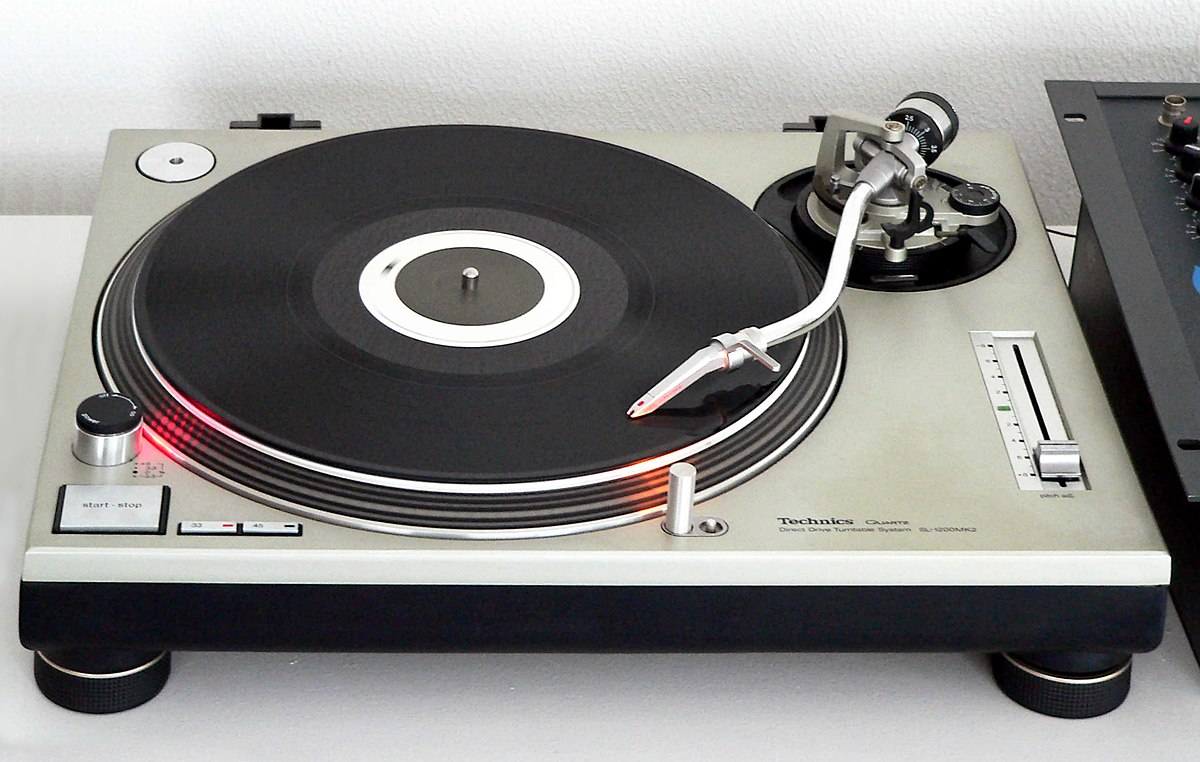
\includegraphics[scale=0.25]{figuras/fig14.png}
	\caption{toca-disco SL-1200 \cite{wikimediaFileTechnicsSL1200MK22jpg}}
	\label{fig14}
\end{figure}

A partir de uma colaboração entre duas gigantes da indústria da música, a \textit{Sony} e a \textit{Philips} criaram o CD em 1979, uma nova mídia capaz de armazenar e reproduzir músicas de forma extremamente compacta, leve e mais barata do que o vinil. No ano seguinte, a mesma colaboração desenvolveu o \textit{Red Book Audio}, o formato de arquivo utilizado no CD, que emprega PCM (\textit{Pulse Code Modulation}) na sua codificação. Esses avanços culminaram em 1982 com o início do consumo de CDs, que popularizou ainda mais o consumo de música ao redor do mundo.

Em 1986, a empresa Rane criou um mixer, visto na Figura \ref{fig15}, focado para \textit{DJs} cuja qualidade se aproximava bastante daquela praticada em estúdios de música: o \textit{MP 24 DJ Club Mixer}. Este desenvolvimento possibilitou um aumento significativo na qualidade do som reproduzido em clubes.

\begin{figure}[h]
	\centering
    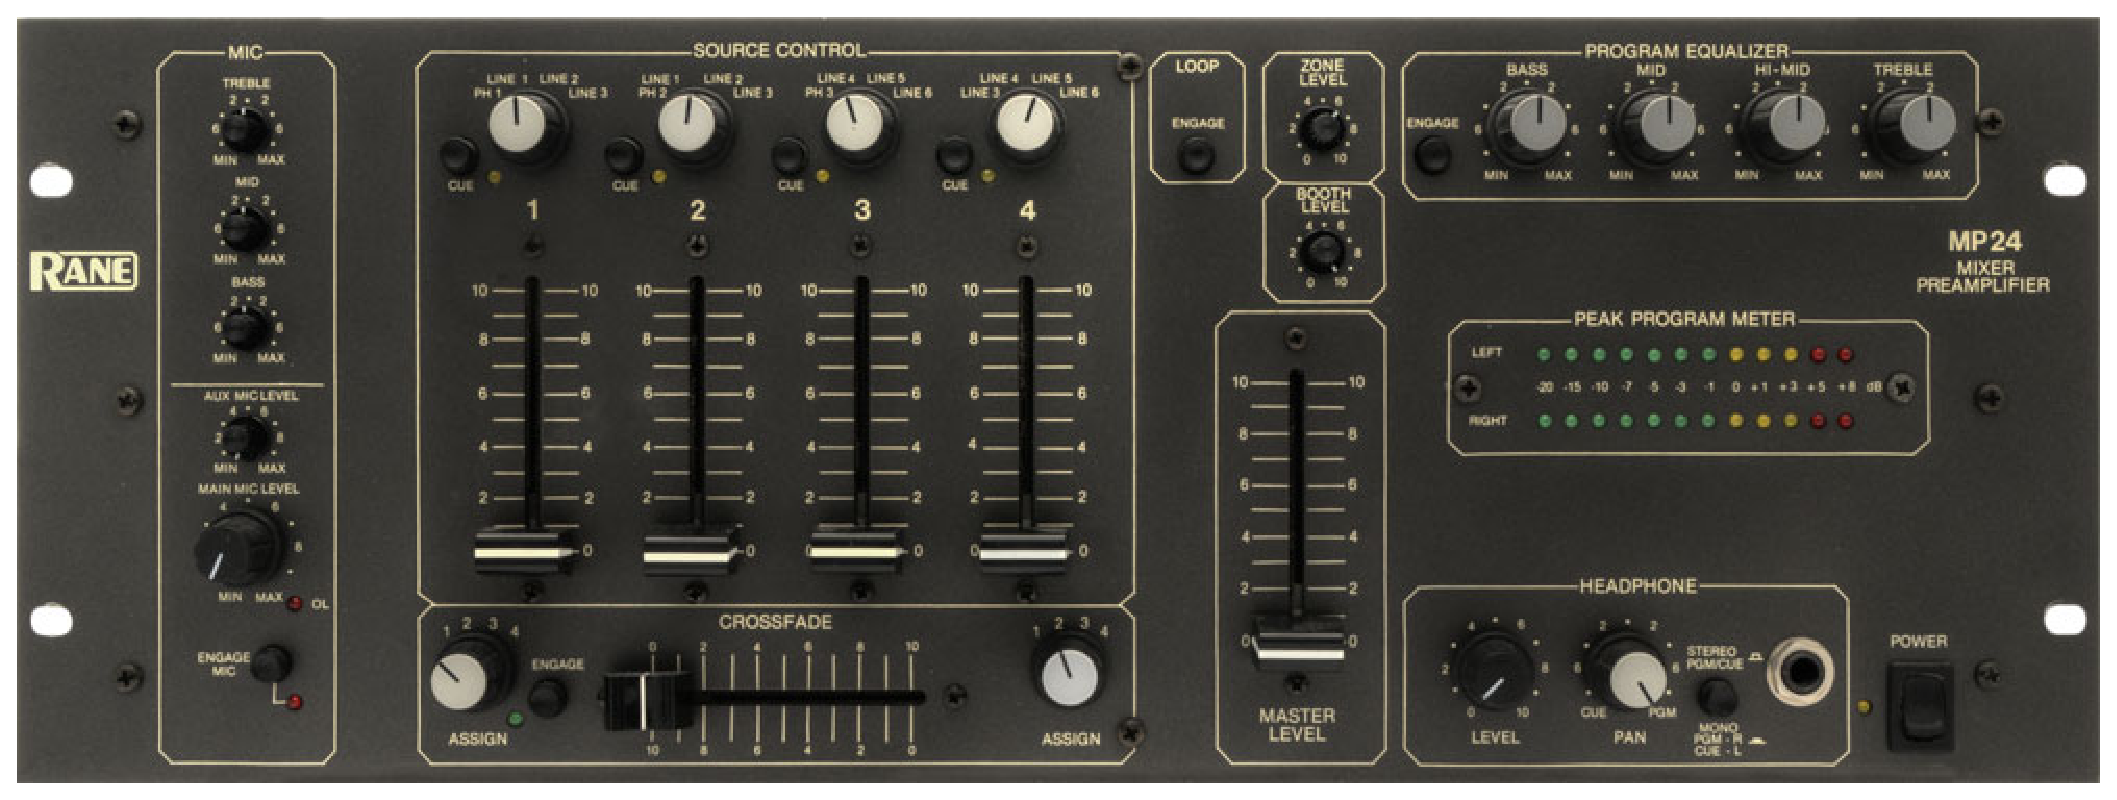
\includegraphics[scale=0.3]{figuras/fig15.eps}
	\caption{mixer criado pela Rane \cite{ranecommercialMixerEvolution}}
	\label{fig15}
\end{figure}

Em 1991, conforme Brewster e Broughton \cite{lastnight}, foi criado o MP3, um formato que permitiu a compressão de arquivos de áudio, eliminando conteúdo redundante. Rapidamente, esse método possibilitou o compartilhamento massivo de músicas pela internet.

Nos anos 90, a \textit{Pioneer}, que viria a se tornar uma gigante no mercado de equipamentos para \textit{DJs}, começou a lançar uma série de produtos que facilitavam e ampliavam a atividade do \textit{DJ}. Em 1992, a empresa lançou a primeira CDJ, um equipamento que integrava várias funções necessárias à mixagem, com suporte para CD. Em 2001, a \textit{Pioneer} lançou uma CDJ com leitor de cartões de memória, e em 2007, uma CDJ capaz de ler dispositivos USB. Isso permitiu que \textit{DJs} não precisassem mais carregar toda a sua discografia, bastando um dispositivo de memória digital para ter sua coleção à disposição.

\begin{figure}[h]
	\centering
    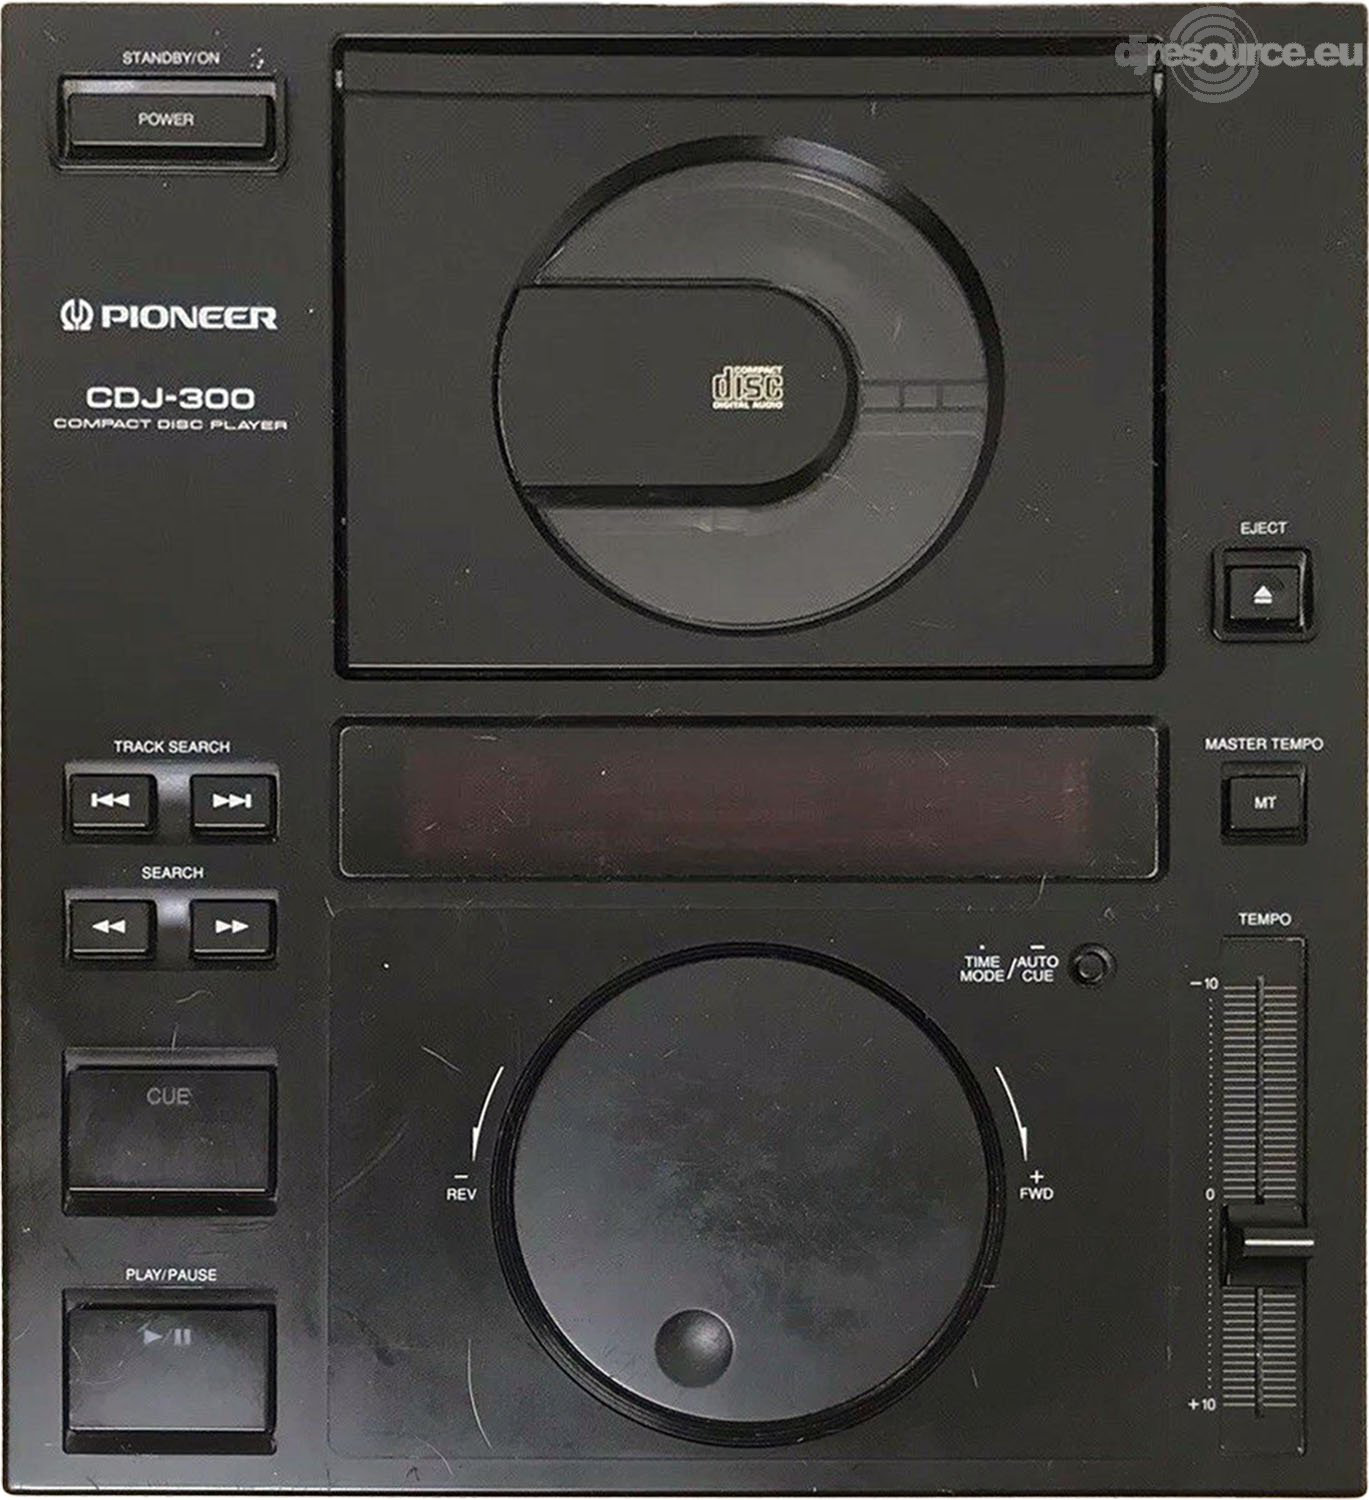
\includegraphics[scale=0.15]{figuras/fig13.eps}
	\caption{CDJ-300 - primeira CDJ da \textit{Pioneer} \cite{cdj300}}
	\label{fig13}
\end{figure}

Na década de 2010, grandes empresas possibilitaram que \textit{DJs} tocassem músicas armazenadas na nuvem e disponíveis em plataformas de streaming. Em 2024, a \textit{Apple} lançou o \textit{Vision Pro}, um óculos de realidade aumentada capaz de emular equipamentos de \textit{DJ}. Com o \textit{Vision Pro}, um \textit{DJ} pode demonstrar suas habilidades e sua coleção com apenas um óculos de VR. Esse equipamento pode ser visto na Figura \ref{fig16}.

\begin{figure}[h]
	\centering
    \includegraphics[scale=0.3]{figuras/fig16.eps}
	\caption{mixagem virtual com o \textit{Apple Vision Pro}o \cite{macmagazineDesenvolvedorFala}}
	\label{fig16}
\end{figure}

Apesar das muitas soluções inovadoras para mixagem, a configuração mais comum atualmente é composta por duas CDJs e um \textit{mixer}, como mostrado na Figura \ref{fig17}.

\begin{figure}[h]
	\centering
    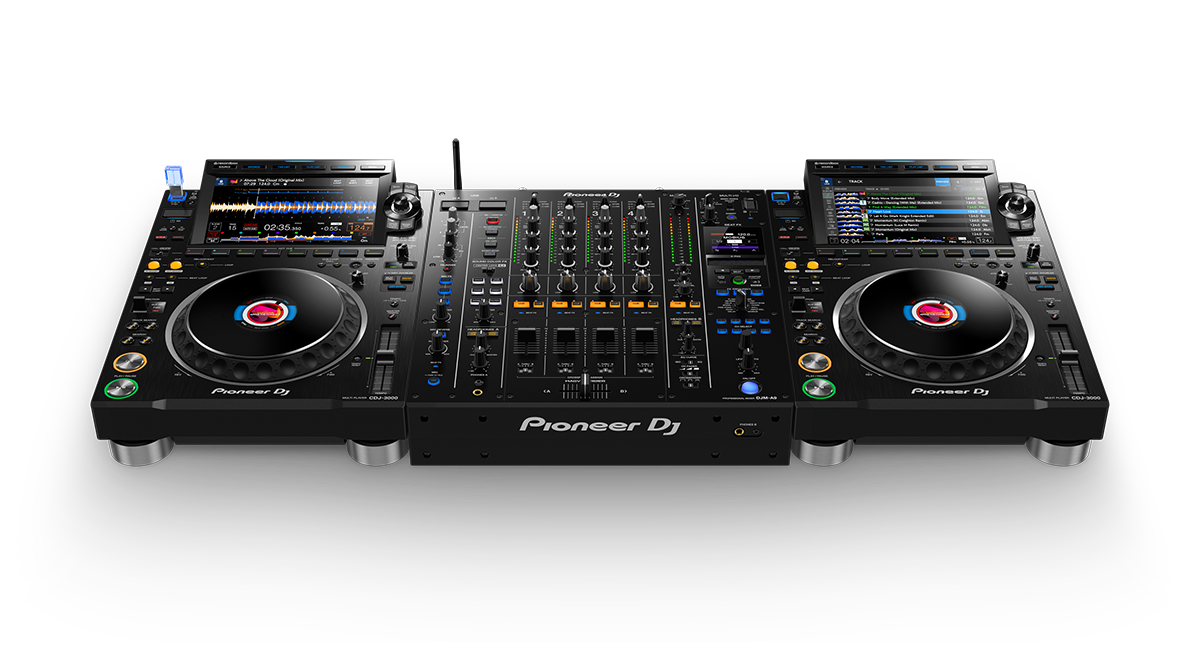
\includegraphics[scale=0.3]{figuras/fig17.png}
	\caption{configuração mais encontrada \cite{pioneerdjDJMA94channel}}
	\label{fig17}
\end{figure}

No entanto, ainda existem configurações que priorizam a qualidade sonora. Para esse público, continuam sendo produzidos equipamentos analógicos que remetem aos \textit{layouts} de \textit{mixers} \textit{vintage}, como os \textit{rotary mixers}, apresentados na Figura \ref{fig18}.

\begin{figure}[h]
	\centering
    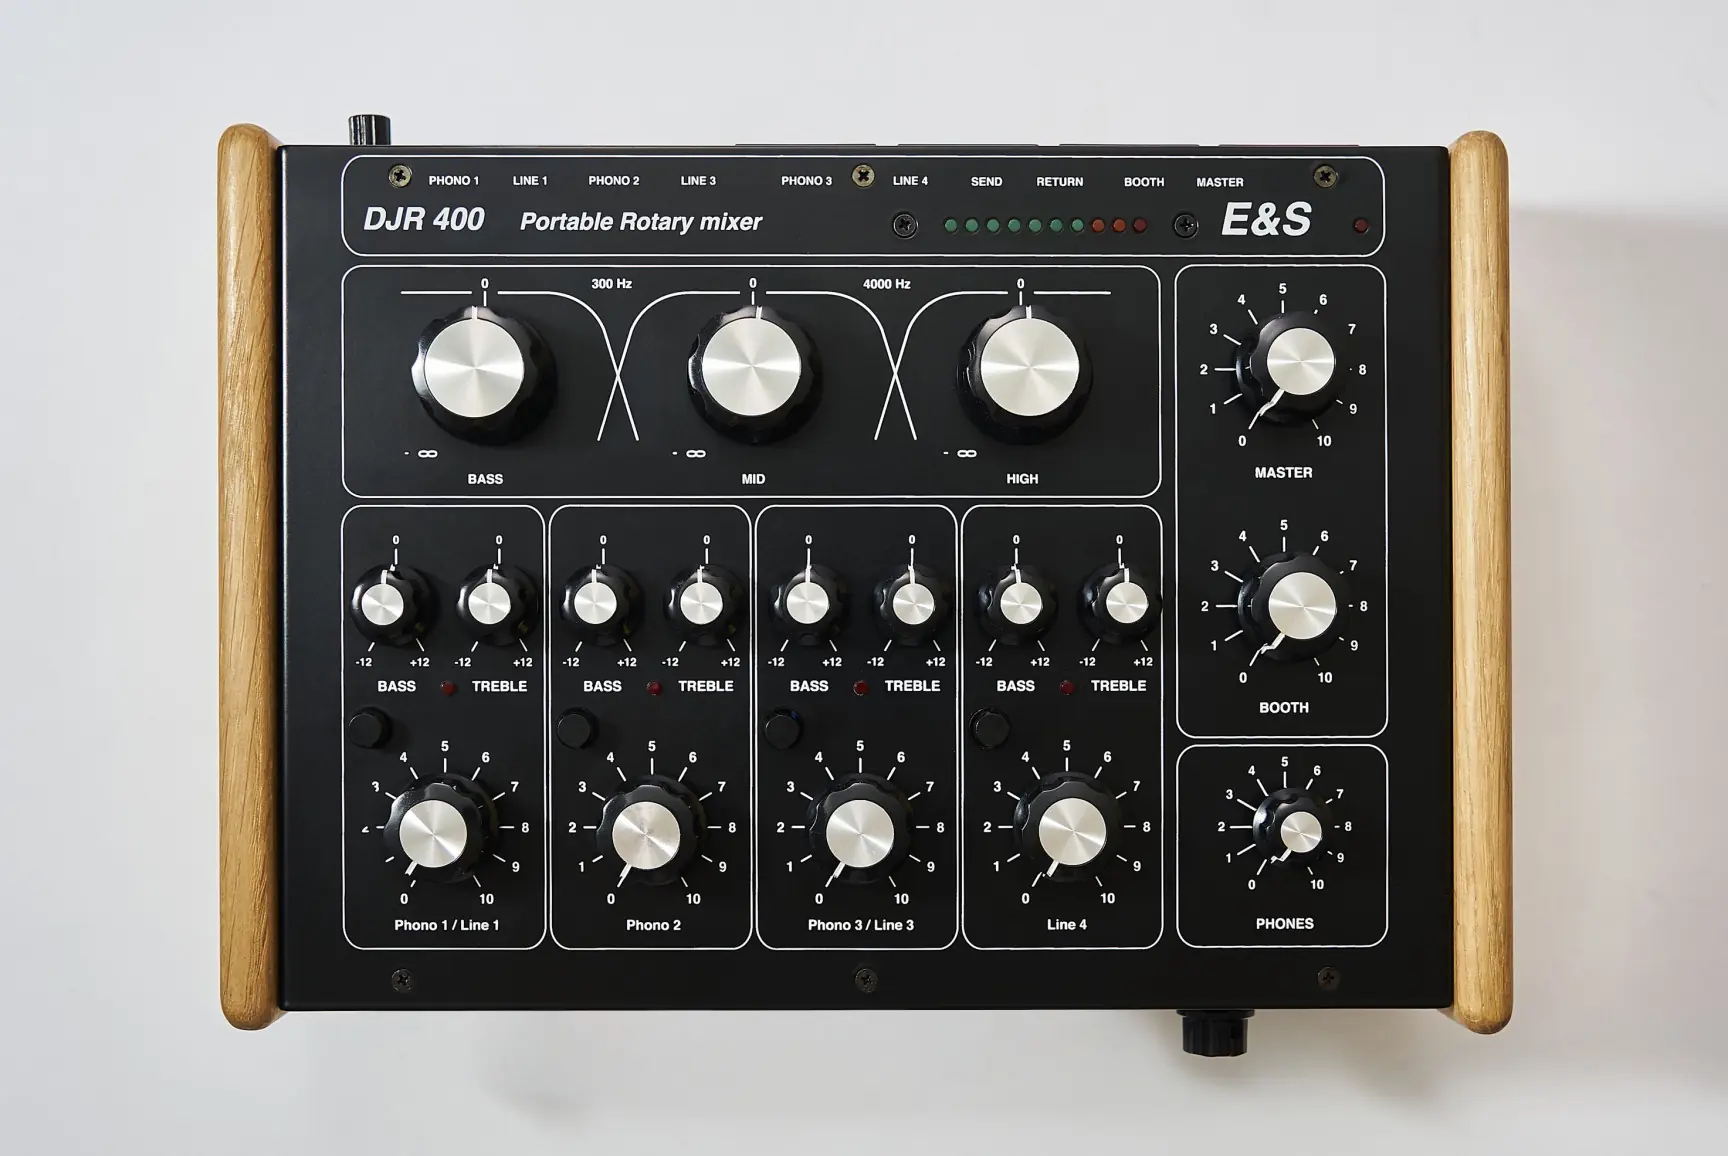
\includegraphics[scale=0.2]{figuras/fig18.png}
	\caption{\textit{rotary mixer} \cite{electroniquespectacleampAUDIO}}
	\label{fig18}
\end{figure}

A mixagem não se limita ao entretenimento em clubes. O papel de um curador musical remonta à época das rádios. Com a evolução da tecnologia de reprodução, armazenamento e gravação de música, a curadoria musical se tornou mais acessível.

A mixagem transcende a mera função de entretenimento. Desde a expansão do conceito de música proposta por John Cage \cite{cage}, no qual música se torna qualquer som, houve várias expansões conceituais tanto teóricas quanto práticas. Uma \textit{mix} pode ser tanto o ato de um produtor musical ponderar a presença de cada instrumento ou canal em uma música quanto o ato de criar uma nova música a partir de várias, resultando em uma colagem sonora.

Uma \textit{mix} possui estrutura e enredo, com início, meio e fim, e serve a diversos propósitos como entretenimento, relaxamento, meditação, cura, dança, apreciação e pesquisa, entre outros. Além disso, os ambientes de circulação são variados, incluindo páginas de \textit{streaming}, festivais, festas e até mesmo sessões individuais de \textit{bedroom djing} (\textit{DJs} que tocam em sua própria casa, geralmente aprendendo a mixar). Nesse cenário, a liberdade do criador se estende para incluir não apenas misturas de músicas de diferentes gêneros, mas também a incorporação de trechos de áudio de entrevistas, livros, filmes, paisagens sonoras e arte sonora, resultando em uma experiência única.

Além disso, a adição de performances ao vivo, com a utilização de sintetizadores e qualquer dispositivo capaz de gerar som, amplia ainda mais as possibilidades criativas. Desde o uso de sinais elétricos provenientes de eletrodos até a integração de elementos inusitados, como performances ao vivo, as opções são verdadeiramente infinitas, limitadas apenas pela imaginação do criador.

\subsection{Parâmetros físicos}

Quando um \textit{DJ} mixa músicas, diversos parâmetros devem ser considerados durante a execução de uma música ou no momento da transição entre duas, como batidas por minuto (BPM), tom, volume, ganho e a presença de componentes em bandas de frequência, como graves, médios e agudos.

A evolução dos equipamentos para \textit{DJs} pode ser descrita pelo aprimoramento do controle de cada um desses parâmetros, visando um design que permita decisões  rápidas com a menor latência possível na saída de áudio e, ao mesmo tempo, melhore o processamento do áudio para obter a melhor qualidade possível.

Para criar uma atmosfera musical ideal, o controle das bandas de frequência é crucial. Ele permite a adição e a subtração de elementos de uma música para criar uma nova versão, que pode ser usada durante a transição entre músicas ou para dar uma nova roupagem a uma música existente. Por exemplo, pode-se adicionar batidas a uma música que não as possui ou adicionar vocal a uma música que é somente instrumental.

O equalizador foi criado, segundo Izhaki \cite{mixing}, pelos \textit{Bell Labs} com o objetivo de ajustar o que era transmitido ao ouvido devido à atenuação de altas frequências durante a transmissão do sinal pelos fios. No entanto, para a produção musical, o equalizador é utilizado para manipular o conteúdo das bandas de frequências dos diversos elementos musicais. A Figura \ref{fig09} ilustra os dois tipos de divisões de bandas apresentados.

\begin{figure}[h]
	\centering
    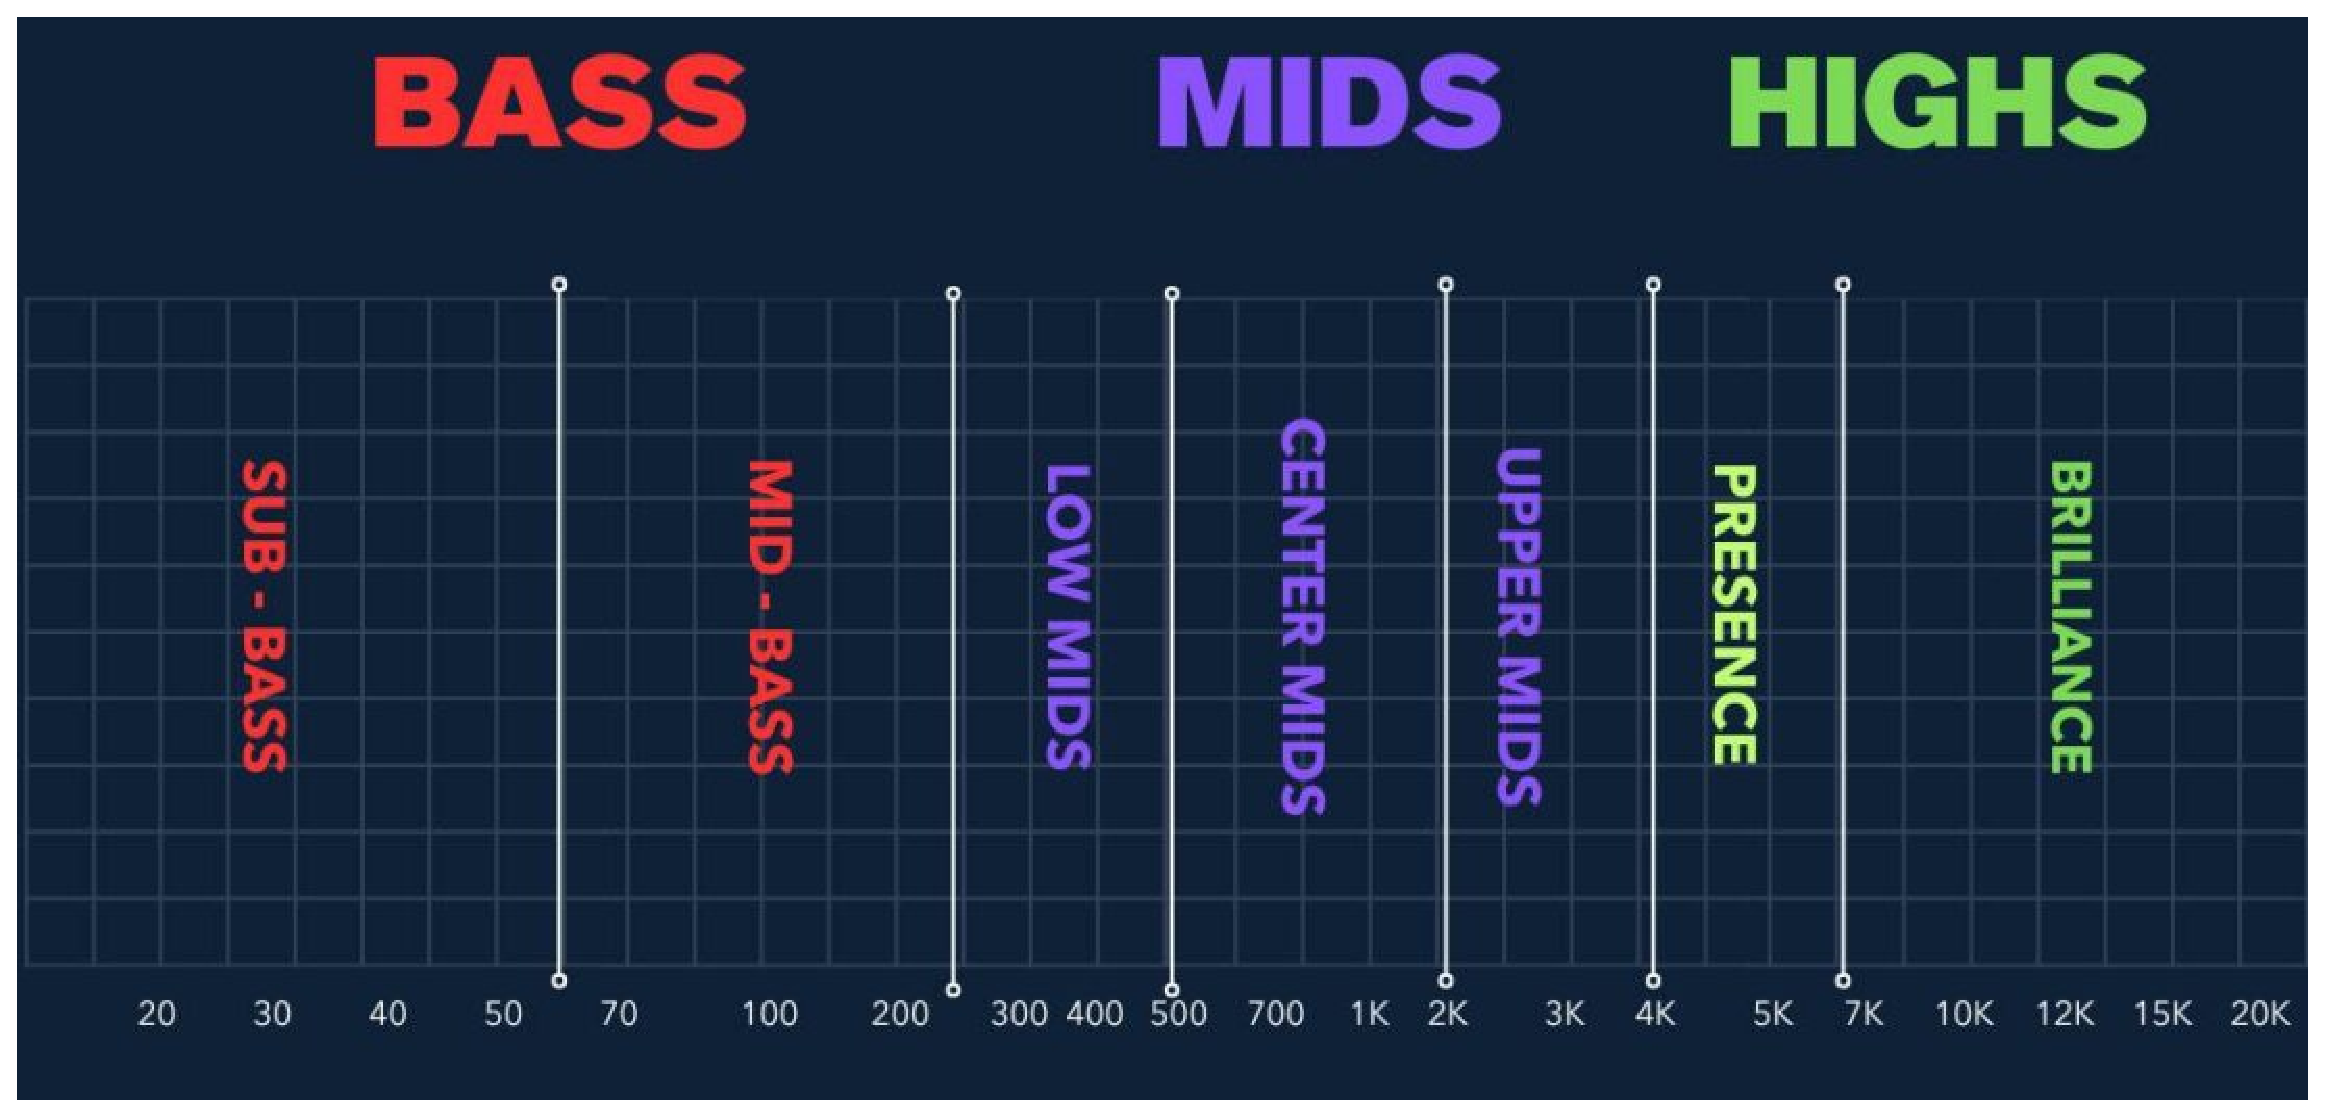
\includegraphics[scale=0.4]{figuras/fig09.eps}
	\caption{Espectro de áudio \cite{headphonestyAudioFrequency}}
	\label{fig09}
\end{figure}

Para a produção musical, considera-se a equalização em sete bandas:

\begin{itemize}
	\item Subgrave: entre 20 e 60 Hz, onde estão elementos como bumbo e baixo.
	\item Graves baixos: entre 60 e 120 Hz, tonalidades associadas ao bumbo e ao baixo.
	\item Médios graves: entre 120 e 250 Hz, onde estão as frequências fundamentais que definem os tons naturais dos instrumentos.
	\item Médios: entre 250 Hz e 2 kHz, onde estão os harmônicos de baixa ordem de vários instrumentos.
	\item Médios altos: entre 2 e 6 kHz, onde há harmônicos complexos.
	\item Agudos ou Brilho: entre 9 e 20 kHz, onde há pouca energia para muitos instrumentos, mas essa banda é importante por estar associada ao brilho na música.
\end{itemize}

A quantidade de bandas e a definição dos intervalos podem variar entre teóricos e equipamentos, portanto, esses intervalos não são uma regra fixa. No entanto, para \textit{DJs}, a maioria dos equipamentos divide o espectro de áudio em três bandas: graves (de 20 a 250 Hz), médios (de 250 Hz a 4 kHz) e agudos (de 4 kHz a 20 kHz).

Essa escolha de bandas reduzidas deve-se à necessidade de simplicidade e rapidez no uso, além de que, em cada uma dessas três bandas, há elementos semelhantes bem definidos, que auxiliam na construção de uma boa mixagem.



\subsubsection{Equipamentos}

Os equipamentos utilizados por \textit{DJs} evoluíram significativamente ao longo do tempo. Inicialmente, utilizavam-se equipamentos improvisados para outras finalidades até que dispositivos específicos para mixagem foram desenvolvidos.

Existem inúmeras configurações possíveis para realizar uma mixagem, e a escolha dos equipamentos depende da fonte de música utilizada. Se a fonte for vinis, devem ser usados toca-discos. Se a fonte for um dispositivo de memória digital, como um pendrive ou cartão de memória, que armazena músicas organizadas por um \textit{software} de gerenciamento, deve-se utilizar uma CDJ. Para performances ao vivo, onde o \textit{DJ} produz música em tempo real, podem ser utilizados \textit{notebooks}, sintetizadores, \textit{samplers}, sequenciadores e muitos outros dispositivos especializados.

\section{Mixer}

Um dispositivo fundamental em qualquer \textit{layout} de mixagem é o \textit{mixer}, cuja função é misturar e controlar os canais de entrada de áudio. Embora existam várias possibilidades de controle, a mais comum é o ajuste das bandas de frequência para cada canal de entrada. Cada dispositivo de reprodução de música é considerado um canal de entrada. O \textit{mixer} é capaz de controlar essas bandas de frequência, bem como somar os sinais de áudio para gerar um sinal de saída que é enviado para os alto-falantes.

Os critérios para classificar um \textit{mixer} como bom são bastante subjetivos. Eles podem incluir o design do equipamento, a qualidade do áudio, a distorção do som, a precisão dos controles, a ergonomia, a portabilidade, o preço, os recursos adicionais como efeitos, referências históricas, e a integração com \textit{software} ou outros equipamentos. Além disso, as preferências pessoais do \textit{DJ} e seu estilo de mixagem influenciam quais aspectos são mais valorizados.

De acordo com Winer \cite{winer}, o desenvolvimento da conexão entre dispositivos de áudio deve considerar três aspectos principais: o sinal de áudio, as impedâncias (de entrada e saída), e o tipo de conector.

\subsection{Potência de Sinal de Áudio}

É comum encontrar entradas \textit{phono} em \textit{mixers}, destinadas a dispositivos como toca-discos, que emitem sinais na ordem de miliVolts. Esses sinais precisam ser amplificados por um amplificador de potência antes de serem processados pelo sistema do \textit{mixer}. Alguns dispositivos têm uma tensão de saída tão baixa que requerem um pré-amplificador para elevar o sinal ao nível de linha adequado para amplificação adicional.

Outra entrada comum é a \textit{line}, que já apresenta sinais em nível de linha. Segundo Winer \cite{winer}, esses sinais possuem dois níveis padrão: -10 dBV para equipamentos não balanceados e +4 dBu para equipamentos balanceados. Equipamentos de linha profissional geralmente são balanceados, com tensões RMS em torno de 1,23 V, enquanto equipamentos não balanceados, como aparelhos de som e TVs, têm tensões em torno de 0,316 V.

\subsection{Cabeamento}

Condutores desbalanceados possuem um fio para transmitir o sinal e um terra comum para referência \cite{bartlett}. A Figura \ref{fig12} ilustra a transmissão de um sinal com ruído através de cabos desbalanceados.

\begin{figure}[h]
	\centering
    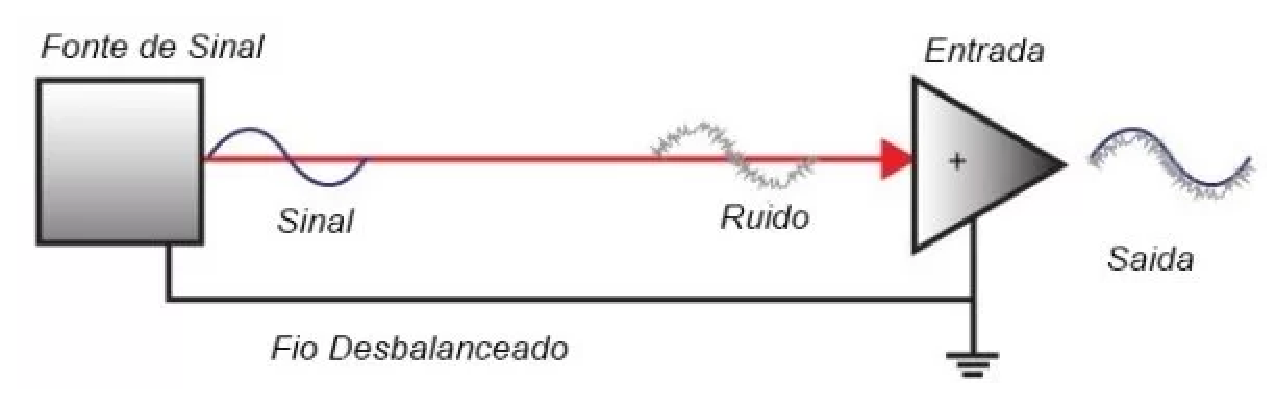
\includegraphics[scale=0.4]{figuras/fig11.eps}
	\caption{transmissão com fio desbalanceado \cite{proaudiospQualDiferena}}
	\label{fig12}
\end{figure}

Por outro lado, condutores balanceados utilizam dois condutores para transmitir o sinal, cobrindo-os com uma blindagem. Ao final da transmissão, um diferenciador é usado para reduzir o ruído adquirido durante a transmissão \cite{bartlett}.

\begin{figure}[h]
	\centering
    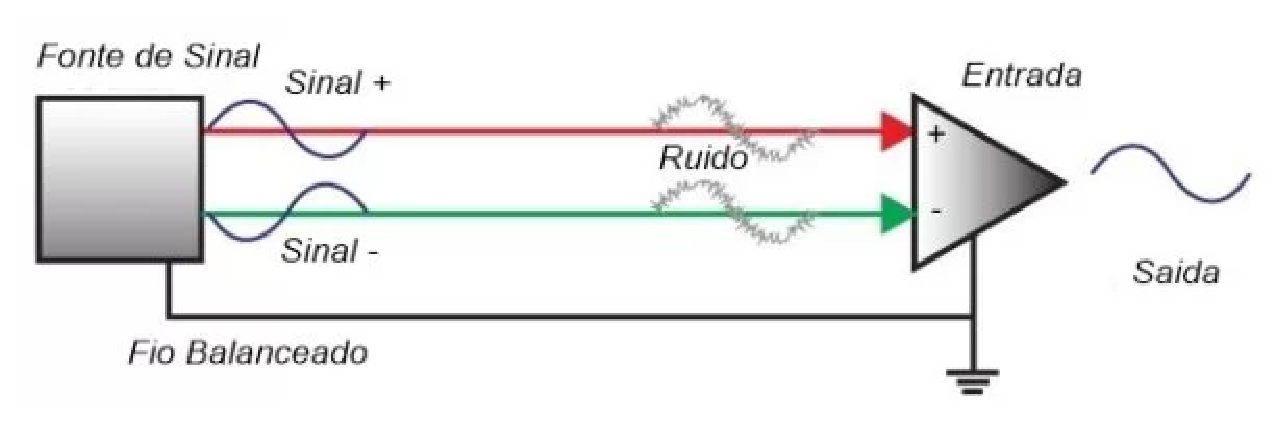
\includegraphics[scale=0.4]{figuras/fig12.eps}
	\caption{esquemático de fio balanceado \cite{proaudiospQualDiferena}}
	\label{fig11}
\end{figure}

A Figura \ref{fig11} mostra um esquemático de fios balanceados no qual há a presença de um condutor adicional, diferente do desbalanceado. 

\subsection{Conectores de 1/4", 1/8" (3,5 mm) e 2,5 mm}

Para conectar dispositivos, é necessário considerar tanto a transmissão de sinais elétricos quanto os conectores. Cada tipo de conector tem suas vantagens relacionadas a aspectos como quantidade de canais, distância, potência, blindagem e interferência.

\begin{figure}[h]
	\centering
    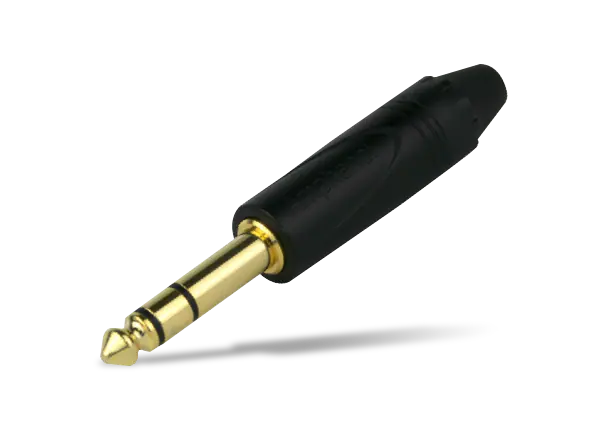
\includegraphics[scale=0.2]{figuras/fig19.png}
	\caption{plug de 1/4" \cite{mouser}}
	\label{fig19}
\end{figure}

Um dos conectores mais conhecidos é o \textit{1/4"} (Figura \ref{fig19}), amplamente utilizado em instrumentos como guitarras, violões e teclados, além de amplificadores e \textit{mixers}. Este conector pode ser usado para sinais estéreos não balanceados ou sinais mono balanceados \cite{bartlett}.

\begin{figure}[h]
	\centering
    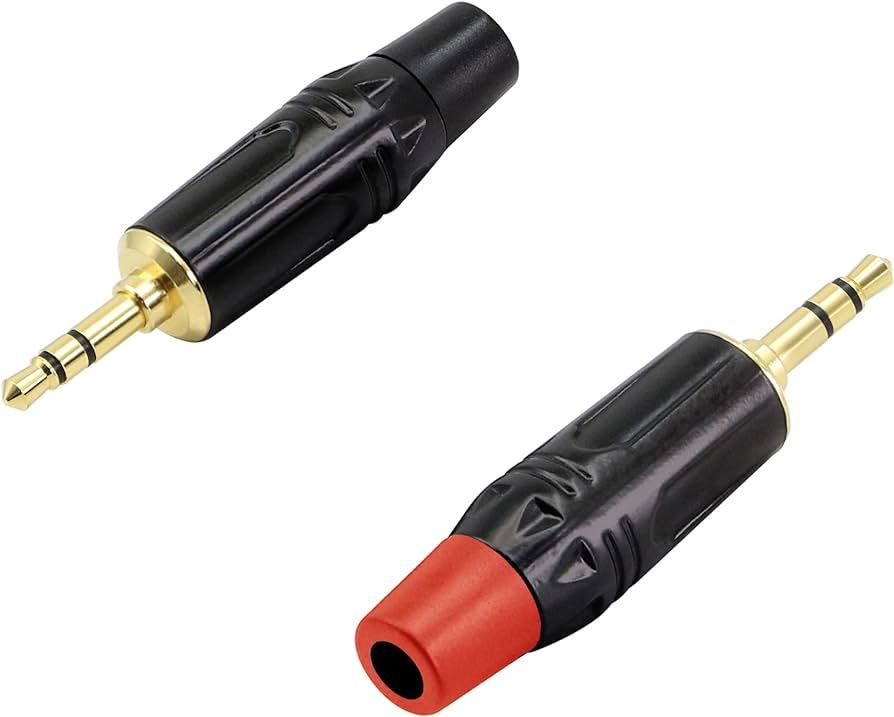
\includegraphics[scale=0.2]{figuras/fig20.png}
	\caption{plug de 1/8" \cite{mouser}}
	\label{fig20}
\end{figure}

O conector \textit{1/8"} (Figura \ref{fig20}), também conhecido como 3,5 mm, é muito encontrado em celulares, dispositivos de reprodução de música e alto-falantes. Internamente, ele possui a mesma construção do conector de 1/4" e pode transmitir os mesmos tipos de sinais.

\begin{figure}[h]
	\centering
    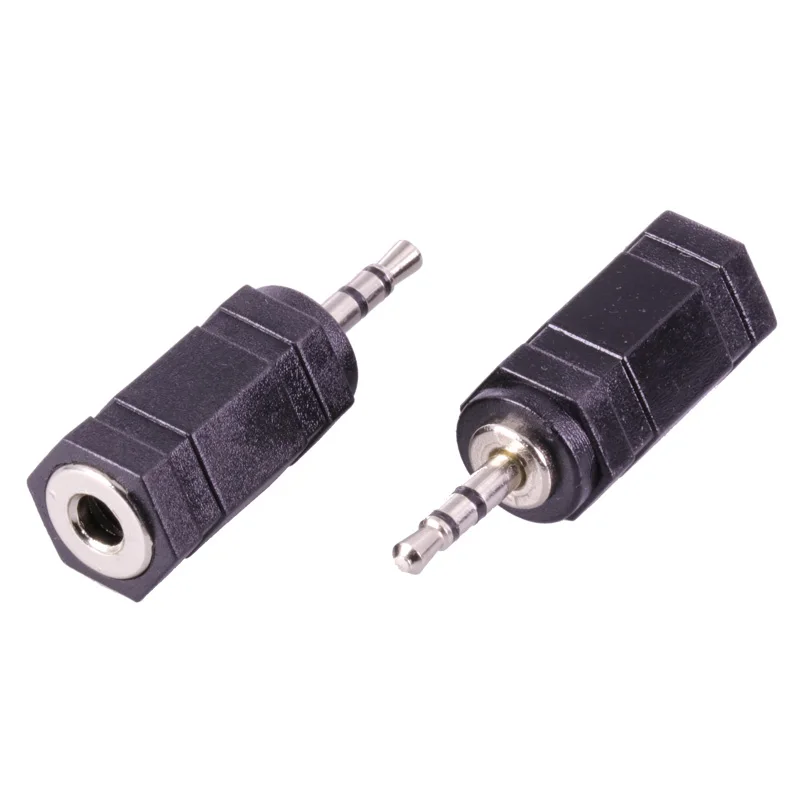
\includegraphics[scale=0.2]{figuras/fig21.png}
	\caption{plug de 2,5 mm \cite{mouser}}
	\label{fig21}
\end{figure}

O conector de 2,5 mm, frequentemente utilizado em \textit{headsets} para adicionar um microfone, possui três fios em vez de dois. A Figura \ref{fig21} ilustra esse tipo de conector.

\subsection{RCA}

O cabo RCA (Figura \ref{fig22}), amplamente utilizado nos primórdios dos sistemas de telefonia e também conhecido como \textit{phono} devido ao seu uso em toca-discos, pode transmitir sinais de áudio mono de forma não balanceada. Para transmitir um sinal estéreo, são usados dois cabos RCA.

\begin{figure}[h]
	\centering
    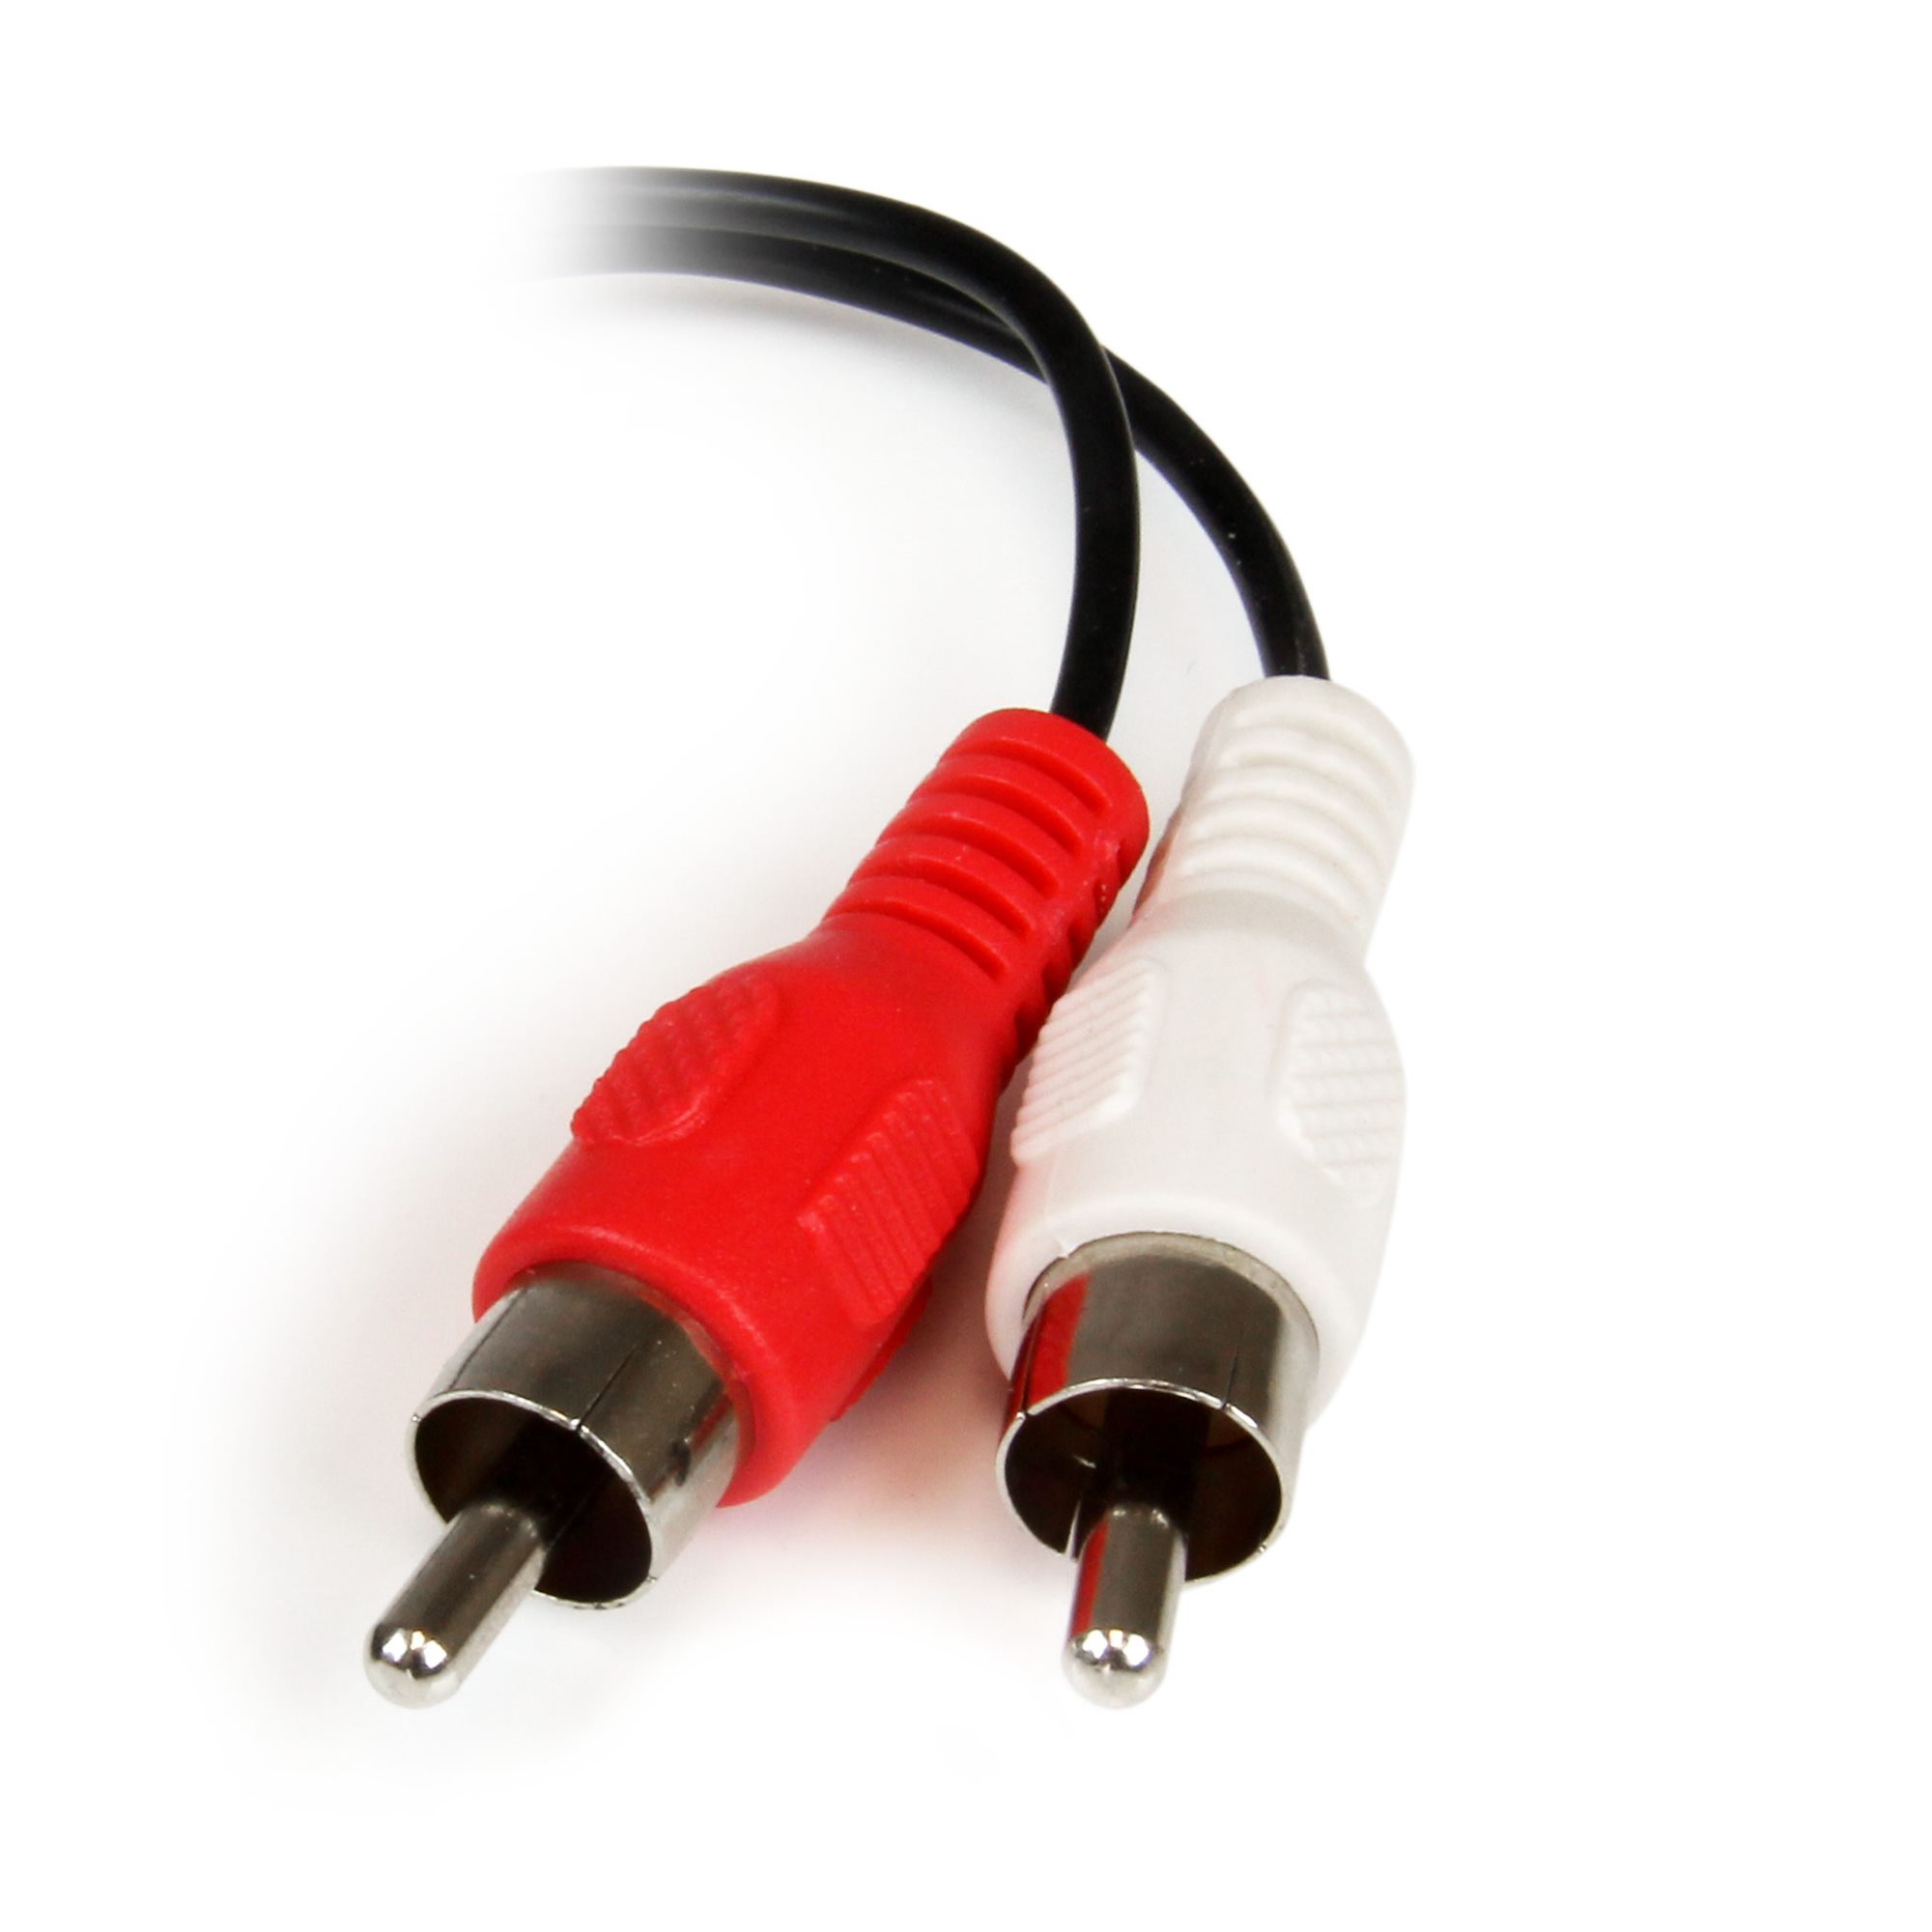
\includegraphics[scale=0.1]{figuras/fig22.png}
	\caption{cabo RCA \cite{rs}}
	\label{fig22}
\end{figure}

Caso um cabo RCA (Figura \ref{fig22}) mono seja conectado, ele pode ser automaticamente duplicado para os dois canais, permitindo que o sinal mono seja transmitido por ambos os canais de áudio \cite{bartlett}.

\subsection{XLR}

O conector XLR, inicialmente chamado de Cannon, foi desenvolvido pela empresa Cannon para a transmissão de sinais balanceados em aplicações profissionais, oferecendo boa rejeição a ruídos e mantendo a integridade do sinal.

\begin{figure}[h]
	\centering
    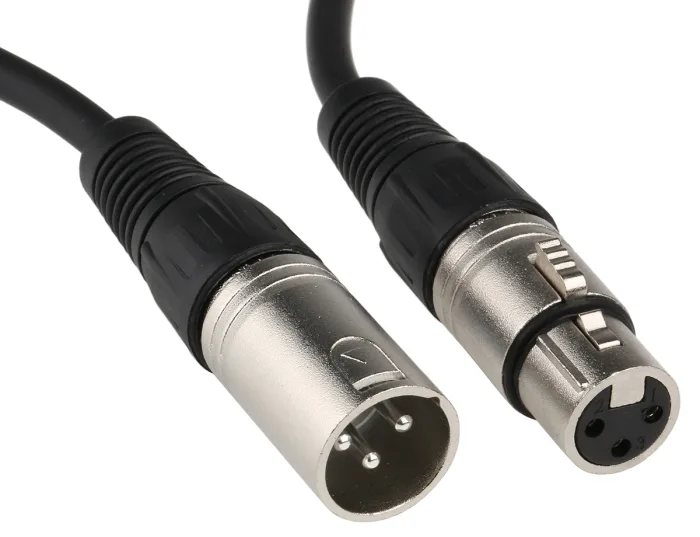
\includegraphics[scale=0.2]{figuras/fig23.png}
	\caption{Conector XLR}
	\label{fig23}
\end{figure}

A Figura \ref{fig23} mostra esse conector, que é amplamente utilizado em áudio profissional, especialmente em microfones, mesas de som e outros equipamentos que exigem alta qualidade de sinal.

\subsection{Protocolos Digitais}

Conectores para transmissão de dados digitais são amplamente utilizados em \textit{mixers} e em outros equipamentos de áudio. Conectores como \textit{Ethernet}, USB, \textit{Bluetooth} e MIDI são comuns para diversas configurações e interações entre dispositivos.

\subsection{Amplificação de Potência}

Os principais níveis de tensão e potência conectados a \textit{mixers} são o nível \textit{Phono} e o nível de linha. A tensão do \textit{Phono} varia entre 0,1 e 5 mV, enquanto a tensão de um nível de linha é em torno de 2,0 $V_{RMS}$. Segundo \cite{self2013audio}, é essencial que exista um intervalo adequado de níveis de tensão para garantir que o sinal se comporte corretamente dentro do amplificador. O sinal não deve ser tão baixo a ponto de os ruídos se tornarem mais proeminentes do que o próprio sinal, nem tão alto a ponto de causar saturação após a amplificação. 

Portanto, quando um sinal \textit{Phono} entra em um \textit{mixer}, ele precisa ser amplificado internamente para alcançar um nível de linha adequado.

\subsection{Equalização}

Como discutido anteriormente, as frequências sonoras audíveis podem ser divididas em três grandes bandas: agudos, médios e graves. 

Tradicionalmente, após a amplificação do sinal, o \textit{mixer} permite o controle do ganho ou a atenuação dessas bandas de frequência. Durante o processo de mixagem, diferentes combinações de ganho podem ser ajustadas conforme necessário, e, em um estágio posterior, todos os canais são somados para produzir o sinal final.

\subsection{\textit{Trim} e Volume}
Quanto à amplitude do sinal de áudio, há dois controles que frequentemente estão presentes em \textit{mixers}: \textit{trim} e volume. O \textit{trim} é um controle sobre o ganho que um sinal obtém antes de ser processado pelo \textit{mixer} e passar pelos controles de equalização. Serve para que o usuário consiga ajustar dois tipos de sinais para que apresentem o mesmo nível ou a combinação desejada; uma mais presente que a outra.
\par
Já o volume é geralmente visto em um controle de \textit{fader}. Esse botão serve para controlar a amplitude do sinal enquanto o sinal é equalizado, ou seja, posteriormente à amplificação do sinal.

\subsection{Conversão AD/DA}

No processamento de sinais de áudio, podemos dividir o tipo de processamento em dois grandes blocos: analógicos e digitais. O processamento analógico é realizado por circuitos analógicos, enquanto o processamento digital é feito por computadores, DSPs e outros dispositivos. A principal diferença reside no estado do sinal durante o processamento. Se o sinal é processado em formato analógico, o \textit{mixer} é analógico, e se o processamento é digital, o \textit{mixer} é digital.

Dispositivos que reproduzem música, como CDJs e toca-discos, podem emitir sinais analógicos ou digitais, dependendo do equipamento e da saída utilizada. Portanto, se o \textit{mixer} requer sinais digitais e a saída do reprodutor de música for analógica, é necessário realizar a conversão de analógico para digital e vice-versa.

Da mesma forma, o sinal de saída do \textit{mixer} precisa ser analógico, pois será amplificado e enviado para os alto-falantes. Assim, se o processamento for realizado de forma digital, o sinal deve passar por uma conversão digital para analógico antes de ser amplificado.